
A possible way of detecting dark matter, in particular axions, is through the use of superconducting qubits.

A qubit is defined, in quantum computing, as a two-state quantum-mechanical system. One of the simplest systems that can show quantum properties.

A qubit can be built with very different technologies: some examples include qubits composed of polarized photons, ions and cold atoms. 
\begin{figure}[H]
    \centering
    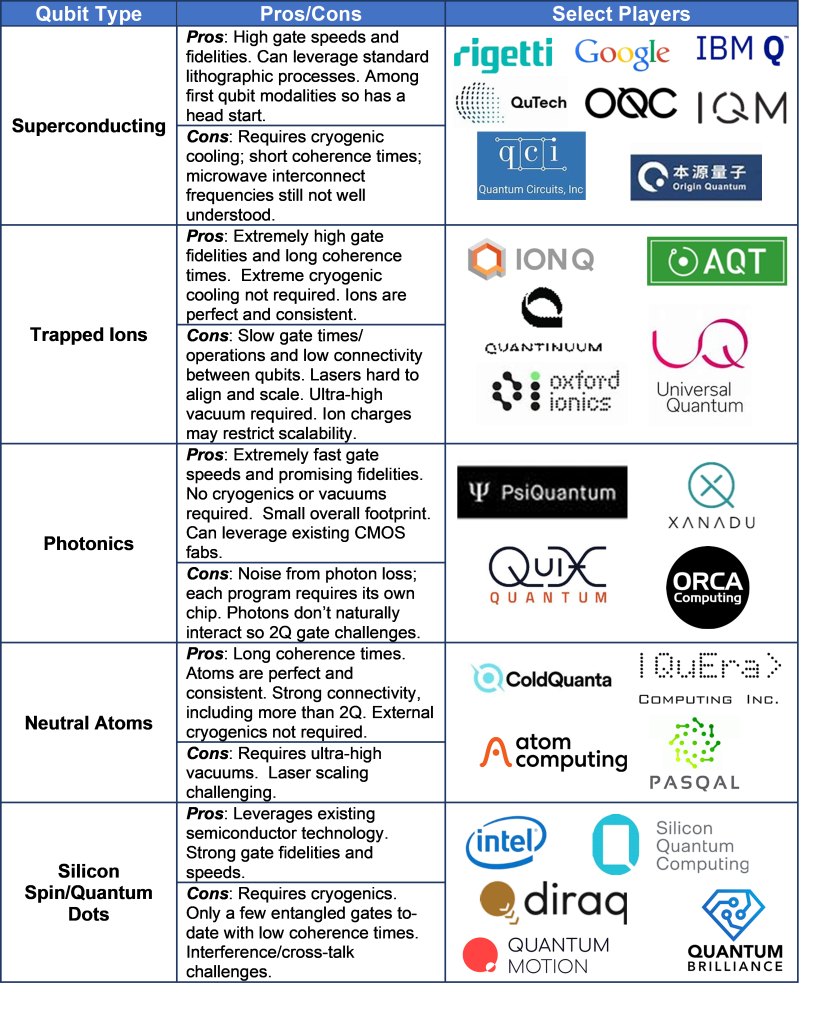
\includegraphics[width=0.8\textwidth]{Theory/figures/qubit_techs.png}
    \caption{Highlight of the main qubit technologies and companies involved in the field. Credits~\cite{quantumtech-blog}.}
    \label{fig:qubit_players}
\end{figure}
In \cref{fig:qubit_players} some of the main companies researching in quantum computing are shown, together with indication on the qubit technology used.
The preferred qubits in the last years were superconducting-based. 
In this thesis, these will be the utilized qubits.


Superconducting qubits are often called artificial atoms and the main idea behind them, is to build a circuit with the first two level very distinguishable from the others. 
So the qubit is obtained by restraining the system.

The superconducting technology has reached very good results~\cite{Arute2019}, but it is still dealing with huge problems also in the hardware and design section.

\subsection{Josephson junction}

To obverse quantum behaviour at a macroscopic level, (so at the size of circuit components), a strong degree of coherence is needed.
In superconducting qubits this is achieved exploiting the phenomenon of superconductivity that is found in some specific metals at cryogenic temperatures~\cite{Tinkham2004}.\\
At these temperatures (i.e. $T\ll T_c$ where $T_c$ is the critical temperature of the material), electrons bound together forming \textit{Cooper pairs} composed of two electrons with equal and opposite momenta~\cite{Langford2013}.
Cooper pairs have a bosonic nature, allowing them to form a condensate, where they are all described by a single quantum ground state, effectively creating a macroscopic quantum phenomenon.
To assure that the number of Cooper pairs remains stable and increase coherence times, superconducting qubits are usually operated below $50$ mK by exploiting complex cryogenics system called cryostat~\cite{Pobell2007}.

The core of a superconducting qubit is the \textit{Josephson junction}~\cite{Kockum2019}: a superconducting inductor that enables the transformation from a harmonic oscillator (standard LC circuit) to an an-harmonic oscillator, needed to separate the 0-1 states and build a qubit.\\
A Josephson junction is composed by a thin insulative gap (order of nm) between two superconductors as presented in \cref{fig:junction}.
The small thickness of the insulator enables the Cooper pairs wavefunction in the two superconductors to overlap, creating a coherent tunneling phenomenon where Cooper pairs can "jump" from one superconductor to the other without any applied voltage.
The resulting current (often referred to as \textit{supercurrent}) has a nonlinear dependence on the voltage applied over the junction, causing the anharmonicity.

\begin{figure}[ht]
    \centering
    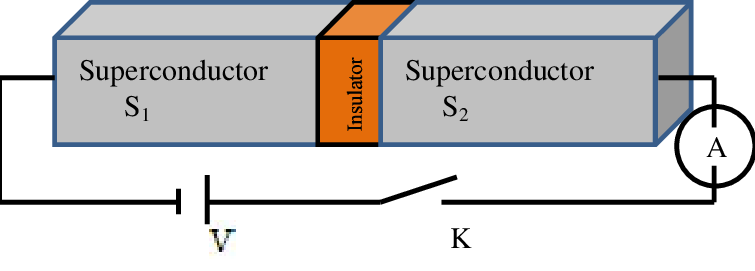
\includegraphics[width=0.6\textwidth]{Theory/figures/josephson_junction.png}
    \caption[Schematic drawing of a Josephson junction]{Schematic drawing of a Josephson junction. Credits~\cite{Vool2017}.}
    \label{fig:junction}
\end{figure}

The Hamiltonian of the Josephson junction can be found from the two equations under the name of \textit{Josephson effect}~\cite{FundamentalsAndFrontiersJosephsonEffect, Josephson1962}:
\begin{align}
    \label{eq:jos_eff_DC}
    I &= I_c \sin \phi \\
    \label{eq:jos_eff_AC}
    \pd{\phi}{t} &= \frac{2e}{\hbar}V
\end{align}
where $I$ is the supercurrent flowing through the junction, $I_c=2eE_J/\hbar$ is the critical current over which the junction starts to exhibit dissipation, $V$ is the voltage applied over the junction and $\phi$, called Josephson phase, is the phase difference between the wavefunction of the two superconductors. 
$E_J$, called Josephson energy, is the energy associated with a single Cooper pair that tunnels through the junction and can be computed as $E_J=L_J I_c^2$ with $L_J=\hbar/2eI_c$ being the inductance of the junction.

The relations expressed in \cref{eq:jos_eff_DC} and \cref{eq:jos_eff_AC} can be used to find the I-V relation:
\begin{equation}
    \pd{I}{t}=\pd{I}{\phi}\pd{\phi}{t} = I_c \frac{2e}{\hbar}V\cos\phi
\end{equation}
That gives an effective inductance term of $L(\phi)=L_J/\cos\phi$ and a inductance Hamiltonian of:
\begin{equation}
    H_L=-E_J\cos\phi
\end{equation}
The physical arrangement of the junction is extremely similar to a parallel plate capacitance and, indeed, this add to the Hamiltonian a capacitive part:
\begin{equation}
    H_C=\frac{Q^2}{2C}=\frac{(2en)^2}{2C} = \frac{4e^2n^2}{2C} = 4E_C n^2
\end{equation}
where we defined the charging energy of a single \textit{electron} as $E_C=e^2/2C$ and $n$ is the number of electron on the capacitor.

Overall, the Hamiltonian of the junction is:
\begin{equation}
    H=H_C+H_L=4E_Cn^2 - E_J \cos \phi
\end{equation}

For now, $n$ and $\phi$ where simple classical variables, now we elevate them to be quantum operators that satisfy the commutator $\left[\hat\phi,\hat n\right]=i$.
For clarity, we will use a \textit{Cooper pair box} (CPB) as system and not a standalone junction~\cite{Bladh2005}. A scheme is presented in \cref{fig:CPB}. 

\begin{figure}[ht]
    \centering
    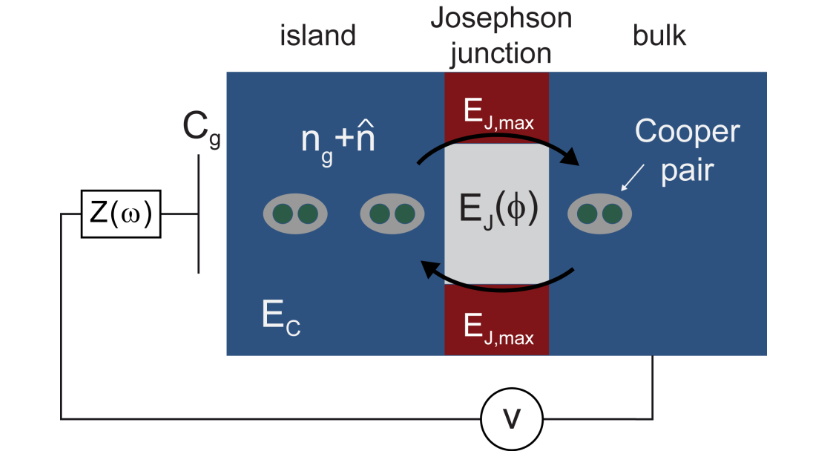
\includegraphics[width=0.6\textwidth]{Theory/figures/CPB.png}
    \caption[Scheme of a Cooper pair box]{Scheme of a Cooper pair box (CPB). Credits~\cite{CPBimage}.}
    \label{fig:CPB}
\end{figure}

The Hamiltonian is almost identical, but we add a $n_g$ term that is the offset charge induced by a voltage source:
\begin{equation}
    H = 4E_C (n-n_g)^2 - E_J \cos\phi \rightarrow  \hat H = 4E_C (\hat n-n_g)^2 - E_J \cos{\hat \phi}
\end{equation}

For a typical CPB we have $E_J/E_C < 1$ so we can express the Hamiltonian in term of \textit{charge states} $\ket N$, namely the eigenstates of $\hat n$ (note that $\left[ \hat H, \hat n \right]=0$).
Note also that with $N$ we indicate the difference of Cooper pairs between the two islands and \textit{not} the total number of Cooper pairs that would be impractical.\\
We can write~\cite{Vool2017}:
\begin{align}
    4E_C(\hat n - n_g)^2 &= 4E_C \sum_N (N-n_g)^2 \ket N \bra N \\
    -E_J \cos{ \hat \phi} &= \frac{E_J}{2}\sum_N (\ket N \bra{N + 1} + \ket{N+1} \bra N)
\end{align}
Note that $\ket N \bra N$ is essentially the number operator for the Cooper pairs, while $\ket N \bra{N+1}$ represents the coherent transfer of a single Cooper pair from island to the reservoir (and the other combination the opposite transfer).

\subsubsection{Flux-tunable Josephson junction}\label{sec:flux_tunable_junction}

A single Josephson junction can be used to build a qubit, but its resonance frequency will be fixed by a relation with $E_J$.
For various reasons, and in particular to achieve two-qubits interactions, it is important to have the capability of "freely" controlling the resonance frequency.

To achieve this tunability, we substitute the Josephson junction with a \textit{superconducting quantum interference device} (SQUID), namely two junctions connected in a loop.
The SQUID, depicted in \cref{fig:squid}, roughly behaves like a single junction, but its Josephson energy is dependent on an external magnetic flux that may run through the loop, thus giving us tunability.

\begin{figure}[ht]
    \centering
    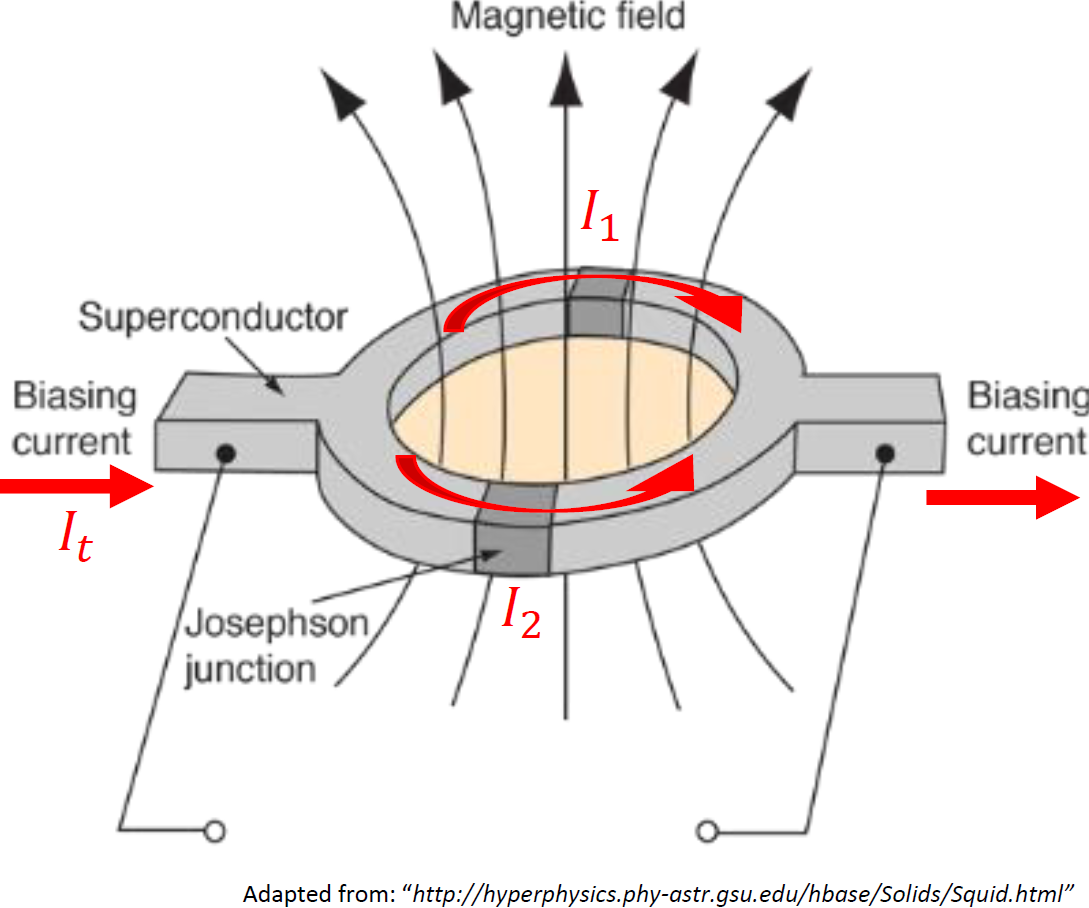
\includegraphics[width=0.5\textwidth]{Theory/figures/squid.png}
    \caption{Schematic layout of a SQUID.}
    \label{fig:squid}
\end{figure}

Let us return to the inductance Hamiltonian (non as an operator), that for a SQUID is:
\begin{equation}
    H_L=-E_J \cos{\phi_1}-E_J \cos{\phi_2}
\end{equation}
where we are assuming that the two junctions are identical (so $E_{J1}=E_{J2}+E_J$).
This simplifies the calculations here, but note that in reality the two energies are purposefully made different to limit the tuning range of the SQUID~\cite{Koch2007}.\\
Between the two phases there is a strict relation:
\begin{equation}
    \phi_1 - \phi_2 = 2\pi l + 2\pi \Phi/\Phi_0
\end{equation}
where we considered two phenomena: the difference in phase, without external flux, must be a multiple of $2\pi$ ($l$ here is an integer) so that the wavefunction is single-valued; and the addition of an external flux $\Phi$ changes the overall phase by a factor dependent on the ration between $\Phi$ and $\Phi_0=h/2e$, the superconducting flux quantum.

So we can now write:
\begin{equation}\label{eq:hl_flux_tunable}
    H_L = -2E_J \cos \left( \frac{\phi_1 - \phi_2}{2} \right) \cos \left( \frac{\phi_1  \phi_2}{2} \right) = -E_{J\Phi} \cos \phi
\end{equation}
where we defined $\phi=(\phi_1 + \phi_2)/2$ and $E_{J\Phi} = 2E_J\cos (\pi \Phi / \Phi_0)$.

So we re-obtain the same exact Hamiltonian form than the simple Josephson junction, but with a tunable $E_J$.